\documentclass[11pt]{article}
\usepackage[left=3.5cm,right=3.5cm,top=2.5cm,bottom=2.5cm]{geometry}
%\usepackage[spanish]{babel}

\usepackage{amsmath,amsfonts,amsthm}
\usepackage{enumitem,mathtools,graphicx}
\setenumerate[0]{label=(\alph*)}

\newtheorem{definition}{Definición}
\newtheorem{exercise}{Ejercicio}
\newtheorem*{sol}{Solución}
\newtheorem*{theorem}{Teorema}

\newcommand\N{\mathbb N}
\newcommand\R{\mathbb R}
\newcommand\C{\mathbb C}

\title{Análisis numérico para ecuaciones diferenciales \\
Tarea 2 - Estabilidad absoluta, ecuaciones en diferencias finitas y
métodos multipaso}
\author{Jorge Alfredo Álvarez Contreras}

\begin{document}
\maketitle

\begin{exercise}
   Se sabe que al aplicar el método de Euler al problema de valores
   iniciales $y'=y$, $y(0)=1$, se obtienen las aproximaciones
   $u_n=(1+h)^{t_n / h}$.
   \begin{enumerate}
     \item
       Demuestre que $y_n-u_n = \frac{1}{2}ht_ne^{t_n}+O(h^{2})$.
     \item
       Usando el resultado anterior, determine el tamaño de paso más
       grande posible para aproximar $y(1)$ con una tolerancia de
       $10^{-5}$. ¿Cuántos pasos de Euler se tienen que dar para
       obtener dicha aproximación de $y(1)$?
   \end{enumerate}
\end{exercise}
\begin{sol}
  Para este problema, supondremos que \emph{primero} se escoge el
  instante de tiempo que será $t_n$ y \emph{después} se escogen $h$ y
  $n$ tales que $t_n$ sea ese instante que se había escogido de
  antemano, de modo que podamos tomar a $t_n$ como una constante dada.
  \begin{enumerate}
    \item
      Dado que $u_n=(1+h)^{t_n/h}$, tenemos
      \begin{align}
        \ln u_n 
        &= \frac{t_n}{h}\ln(1+h) \\
        &= \frac{t_n}{h}\left(h-\frac{h^{2}}{2} + O(h^{3})\right) \\
        &= t_n - t_n \frac{h}{2} + O(h^{2})
      .\end{align}
      Esto significa que tenemos una función $f(h)$, un $h_0>0$ y una
      constante $C>0$ tales que, para todo $0<h<h_0$, se satisfacen
      $|f(h)|\leq Ch^{2}$ y
      \begin{equation}
        \ln u_n = t_n - t_n \frac{h}{2} + f(h)
      .\end{equation}
      Notemos que, para $0<h<h_0$, tenemos
      \begin{align}
         \left| -t_n \frac{h}{2} + f(h) \right|^{2}
         &\leq t_n^{2} \frac{h^{2}}{4} + t_n h |f(h)| + |f(h)|^{2} \\
         &\leq T^{2} \frac{h^{2}}{4} + t_n h Ch^{2} + C^{2}h^{4} \\
         &\leq
         \left(\frac{T^{2}}{4} + t_n h_0 C + C^{2}h_0 \right)h^{2}
      .\end{align}
      Por lo tanto,
      \begin{equation}
         \left( -t_n \frac{h}{2} + f(h) \right)^{2}
         = O(h^{2})
      .\end{equation}
      
       
      Luego,
      \begin{align}
        u_n
        &= e^{t_n}e^{-t_n \frac{h}{2} + f(h)} \\
        &= e^{t_n}
            \left(1
             -t_n \frac{h}{2} + f(h)
             + O\left(\left(
             -t_n \frac{h}{2} + f(h)
             \right)^{2}
             \right)
          \right) \\
        &= 
            e^{t_n}
             -t_n \frac{h}{2}e^{t_n} + O(h^{2})
      .\end{align}
      Ahora, notando que la solución analítica es $y(t)=e^{t}$,
      tenemos $y_n=e^{t_n}$, por lo cual
      \begin{align}
        y_n - u_n
        &= e^{t_n} - u_n \\
        &= t_n \frac{h}{2} e^{t_n} + O(h^{2})
      ,\end{align}
      como se quería.
    \item
      Ahora supongamos que queremos aproximar $y(1)$ con una
      tolerancia de $10^{-5}$. Es decir, aproximando en el intervalo
      $[0,1]$, queremos que
       \begin{equation}
        |y_{N_h}-u_{N_h}| < 10^{-5}
      \end{equation}
      donde $N_h$ es el mayor entero con $hN_h\leq 1$.
      Despreciando el término cuadrático en $h$, esto es
       \begin{equation}
        \frac{1}{2}he < 10^{-5}
      \end{equation}
      o bien,
      \begin{equation}
        h < 2e^{-1}10^{-5}
      .\end{equation}
      Por lo tanto,
      \begin{equation}
        N_h
        = \left\lfloor \frac{1}{h} \right\rfloor
        = \left\lfloor \frac{10^{5}e}{2} \right\rfloor
        = 135914
      .\end{equation}
      En efecto, al aplicar el método con $h=7.3576\cdot 10^{-6}
      \approx 2e^{-1}10^{-5}$ y graficar el error, obtenemos
      \begin{center}
      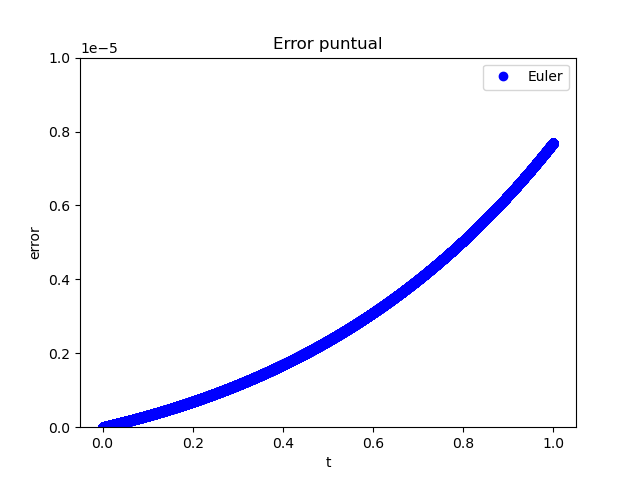
\includegraphics[width=0.7\textwidth]
      {img/jaac_tarea2_ejercicio1.png}
      \end{center}
      aunque esto parece una mera casualidad, ya que al disminuir $h$ 
      (por ejemplo, $h=7.3575\cdot 10^{-6}$, $h=7.3574\cdot 10^{-6}$,
      $h=7.3573\cdot 10^{-6}$, $h=7.3573\cdot 10^{-6}$)
      el error disminuye, vuelve a subir y luego vuelve a bajar.
      Supongo que esto es por problemas de redondeo. Sin embargo, al
      menos el error se mantiene en el mismo orden de magnitud, lo
      cual nos dice que la teoría no está tan mal.
  \end{enumerate}
\end{sol}

\begin{exercise}
  Determine y grafique (con ayuda de \texttt{python}) la región de
  estabilidad absoluta de los métodos
  \begin{enumerate}
    \item
      Heun
    \item
      BDF2
  \end{enumerate}
\end{exercise}
\begin{sol}
  \begin{enumerate}
    \item
      El método de Heun es
      \begin{equation}
        u_{n+1} = u_n + \frac{h}{2}[f_n + f(t_{n+1},u_n+hf_n)]
      .\end{equation}
      Para el problema de prueba $y'=y$, tenemos $f(t,y)=\lambda y$,
      así que
      \begin{align}
        f_n
          &= f(t_n,u_n)
          = \lambda u_n \\
        f(t_{n+1},u_{n}+hf_n)
          &= \lambda(u_{n}+hf_n)
          = \lambda u_n + h\lambda^{2} u_n
      .\end{align}
      Luego, el método es
      \begin{align}
        u_{n+1}
        &= u_n + \frac{h}{2}(2\lambda u_n + h\lambda^{2} u_n) \\
        &= \left(1 + h\lambda + \frac{1}{2}(h\lambda)^{2}\right) u_n
      \end{align}
      con $u_0=1$.
      Por lo tanto, la solución es
      \begin{equation}
        u_n
        = \left(1 + h\lambda + \frac{1}{2}(h\lambda)^{2}\right)^{n}
      .\end{equation}
      y la región de estabilidad absoluta del método consiste en los
      $z\in\C$ tales que
      \begin{equation}
        \left(1 + z + \frac{1}{2}z^{2}\right)^{n} \to 0
      .\end{equation}
      Esto sucede si, y solo si, 
      \begin{equation}
        \left|1 + z + \frac{1}{2}z^{2}\right|^{n} \to 0
      .\end{equation}
      lo cual sucede exactamente cuando
      \begin{equation}
        \left|1 + z + \frac{1}{2}z^{2}\right|^{2}<1
      .\end{equation}
      No pude sacar una forma explícita para esta región pero hice un
      muestreo aleatorio y obtuve la siguiente gráfica:
      \begin{center}
        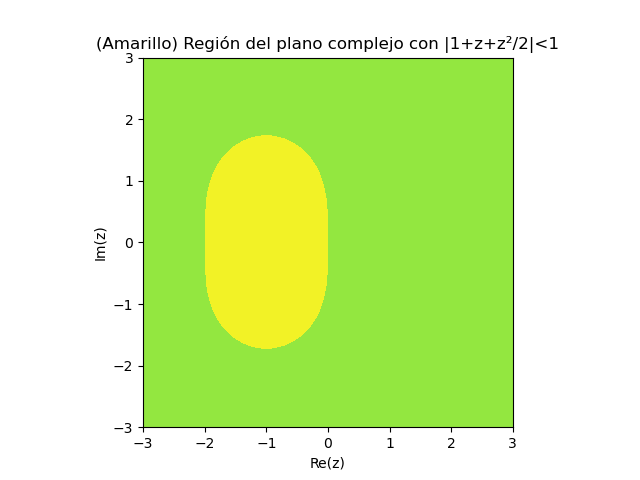
\includegraphics[width=0.7\textwidth]
        {img/jaac_tarea2_ejercicio2a.png}
      \end{center}
        
    \item
      El método BDF2 es
      \begin{equation}
        \frac{1}{2h}(u_{n-1} - 4 u_n + 3 u_{n+1}) - f_{n+1} = 0
      .\end{equation}
      Para el problema de prueba $f(t,y)=\lambda y$, tenemos
      \begin{equation}
        u_{n-1} - 4 u_n + 3 u_{n+1} - 2h\lambda u_{n+1} = 0
      .\end{equation}
      Obtenemos el polinomio característico sustituyendo $u_n$ por
      $r^{n}$ del lado izquierdo y tomando $n=1$:
      \begin{align}
        \pi(r;h\lambda)
        &= 1 - 4 r + 3 r^{2} - 2h\lambda r^{2}
      \end{align}
      % que se puede escribir como
      % \begin{equation}
      %   \pi(r;h\lambda) = \rho(r) - h\lambda \sigma(r)
      % \end{equation}
      % donde
      % \begin{align}
      %   \rho(r) &= 1 - 4 r + 3 r^{2} \\
      %   \sigma(r) &= 2r^{2}
      % .\end{align}
      cuyas raíces son
      \begin{equation}
        r_{0,1}(h\lambda) = \frac{2\pm\sqrt{1+2h\lambda}}{3-2h\lambda}
      \end{equation}
      cuando $h\lambda \neq \frac{3}{2}$.
      Este caso de todos modos lo evitamos, pues buscamos que
      $\Re(\lambda)<0$.
      Dado que la condición absoluta de la raíz es equivalente a la
      estabilidad absoluta, basta encontrar los $z=h\lambda$ tales
      que las raíces $r_{0,1}(z)$ tengan norma menor a $1$.
      De nuevo, hice un muestreo aleatorio y obtuve la siguiente
      gráfica:
      \begin{center}
        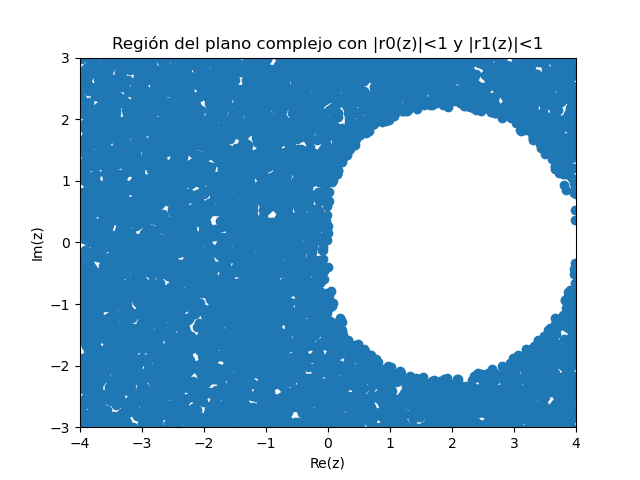
\includegraphics[width=0.7\textwidth]
        {img/jaac_tarea2_ejercicio2b.png}
      \end{center}

  \end{enumerate}
\end{sol}

\begin{exercise}
  Resuelva la ecuación en diferencias
  \begin{equation}\label{eq:problema}
    u_{n+4} - 6u_{n+3} + 14u_{n+2} - 16 u_{n+1} + 8u_{n} = n
  \end{equation}
  con las condiciones $u_0=1$, $u_1=2$, $u_2=3$, $u_3=4$.

  \emph{Solución: $u_n=2^n(n / 4 -1) + 2^{(n-2) / 2}\sin(n\pi /
  4)+n+2$}.
\end{exercise}
\begin{sol}
  Primero resolvamos la ecuación homogénea asociada.
  \begin{equation}\label{eq:homogeneo}
    v_{n+4} - 6v_{n+3} + 14v_{n+2} - 16 v_{n+1} + 8v_{n} = 0
  \end{equation}
  El polinomio característico $\pi(r)$ de la ecuación
  se obtiene tomando el lado izquierdo, sustituyendo $v_n=r^{n}$ y
  poniendo $n=0$:
  \begin{equation}\label{eq:charpol}
    \pi(r) = r^{4} - 6r^{3} + 14r^{2} - 16 r + 8 
  \end{equation}
  Las raíces de este polinomio son
  \begin{align}
    r_{0,1} &= 2  \quad \text{(multiplicidad $2$)}\\
    r_{2,3} &= 1 \pm i
  ,\end{align}
  por lo cual la solución general es de la forma
  \begin{equation}
    v_n
    = (\gamma_0 + \gamma_1 n) 2^{n}
    + \gamma_2(1+i)^{n}
    + \gamma_3(1-i)^{n}
  .\end{equation}
  Ahora encontremos una solución particular $w_n$ de la ecuación
  \eqref{eq:problema}. Claramente, $w_n$ no puede ser una constante
  $w_n=a$, pues en ese caso obtendríamos $a=n$. Entonces intentemos un
  polinomio de grado $1$: supongamos que $w_n=a+bn$. Sustituyendo en
  \eqref{eq:problema} , tenemos
  \begin{equation}
    a+b(n+4) - 6(a+b(n+3)) + 14(a+b(n+2)) - 16(a+b(n+1)) + 8(a+bn) = n
  \end{equation}
  Agrupando los términos constantes y los términos con $n$, obtenemos
  \begin{equation}
    bn + a+4b -18b +28b -16b = n
  \end{equation}
  Luego, $b=1$, por lo cual $a=-4+18-28+16=2$.
  De este modo, obtenemos
  \begin{align}
    u_n
    &= v_n + 2 + n \\
    &= (\gamma_0 + \gamma_1 n) 2^{n}
    + \gamma_2(1+i)^{n}
    + \gamma_3(1-i)^{n}
    + 2
    + n
  .\end{align}
  Imponiendo las condiciones iniciales $u_0=1, u_1=2, u_2=3, u_3=4$,
  obtenemos las ecuaciones
  \begin{align}
    \gamma_0
    + \gamma_2
    + \gamma_3
    &= 1 - 2 - 0
    \\
    2\gamma_0 + 2\gamma_1
    +
    (1+i)
    \gamma_2
    +
    (1-i)
    \gamma_3
    &= 2 - 2 - 1
    \\
    4\gamma_0 + 8\gamma_1
    + 2i \gamma_2
    - 2i\gamma_3
    &= 3 - 2 - 2
    \\
    8\gamma_0 + 24\gamma_1
    + (-2+2i)\gamma_2
    + (-2-2i)\gamma_3
    &= 4 - 2 - 3
  .\end{align}
  En términios matriciales, esto es
  \begin{equation}
    \begin{bmatrix}
      1 & 0 & 1 & 1 \\
      2 & 2 & 1+i & 1-i \\
      4 & 8 & 2i & -2i \\
      8 & 24 & -2+2i & -2-2i
    \end{bmatrix}
    \begin{bmatrix}
      \gamma_0 \\
      \gamma_1 \\
      \gamma_2 \\
      \gamma_3
    \end{bmatrix}
    =
    \begin{bmatrix}
      -1 \\
      -1 \\
      -1 \\
      -1
    \end{bmatrix}
  \end{equation}
  La solución de este sistema es
  \begin{equation}
    \begin{bmatrix}
      \gamma_0 \\
      \gamma_1 \\
      \gamma_2 \\
      \gamma_3
    \end{bmatrix}
    =
    \begin{bmatrix}
      -1 \\
      \frac{1}{4} \\
      -\frac{i}{4} \\
      \frac{i}{4}
    \end{bmatrix}
  .\end{equation}
  Es decir,
  \begin{align}
    u_n
    &= (-1 + n / 4) 2^{n}
    - \frac{i(1+i)^{n} - i(1-i)^{n}}{4}
    + 2 + n
    \\
    &= (n / 4 - 1) 2^{n}
    + \frac{2^{n / 2}e^{i\pi n / 4} - 2^{n / 2} e^{-i\pi n / 4}}{4i}
    + 2 + n
    \\
    &= (n / 4 - 1) 2^{n}
    + 2^{n / 2 - 1} \sin(\pi n / 4)
    + 2 + n
  ,\end{align}
  como se quería.
\end{sol}

\begin{exercise}
  Calcule el error de truncamiento local $\tau_{n+1}(h)$ y la
  constante de error del método de Adams-Moulton AM3.
\end{exercise}
\begin{sol}
  El método es
  \begin{equation}
    u_{n+1} = u_n + \frac{h}{12}(5f_{n+1}+8f_n-f_{n-1})
  .\end{equation}
  Sustituyendo $u_n$ con $y_n$ y $f_n$ con $f(t_n,y_n)=y'_n$,
  obtenemos la ecuación que satisface el error residual:
  \begin{equation}
    y_{n+1}
    = y_n
    + \frac{h}{12}[5y'_{n+1}+8y'_n-y'_{n-1}]
    + \epsilon_{n+1}
  .\end{equation}
  Es decir,
  \begin{equation}
    \epsilon_{n+1}
    = y_{n+1}
    - y_n
    - \frac{h}{12}[5y'_{n+1}+8y'_n-y'_{n-1}]
  .\end{equation}
  Expandiendo hasta orden $4$ en $h$, tenemos
  \begin{align}
    \epsilon_{n+1}
    &= y_n + hy'_n
      + \frac{h^{2}}{2}y''_n
      + \frac{h^{3}}{3!}y'''_n
      + \frac{h^{4}}{4!} y''''_n
      - y_n
    \\
    &\quad
      - \frac{5h}{12}
      \left(
        y'_{n}+hy''_n
        + \frac{h^{2}}{2}y'''_n
        + \frac{h^{3}}{3!}y''''_n
      \right) \\
    &\quad - \frac{8h}{12}y'_n \\
    &\quad
      + \frac{h}{12}
      \left(
        y'_{n}
        - hy''_n
        + \frac{h^{2}}{2}y'''_n
        - \frac{h^{3}}{3!}y''''_n
      \right)
      + O(h^{5})
    \\
    &= \frac{h}{12}
      \left(
        12y'_n
        + 6hy''_n
        + 2h^{2}y'''_n
        + \frac{h^{3}}{2} y''''_n
      \right)
    \\
    &\quad
      + \frac{h}{12}
      \left(
        - 5y'_{n}
        - 5hy''_n
        - \frac{5h^{2}}{2}y'''_n
        - \frac{5h^{3}}{6}y''''_n
      \right) \\
    &\quad
      - \frac{h}{12}8y'_n \\
    &\quad
      + \frac{h}{12}
      \left(
        y'_{n}
        - hy''_n
        + \frac{h^{2}}{2}y'''_n
        - \frac{h^{3}}{6}y''''_n
      \right)
    + O(h^{5})
    \\
    &= -\frac{h^{4}}{24}
      y''''_n
    + O(h^{5})
  .\end{align}
  Por lo tanto, el error de truncamiento local es
  \begin{equation}
    \tau_{n+1} = \frac{\epsilon_{n+1}}{h}
    = -\frac{h^{3}}{24}
      y''''_n
    + O(h^{4})
  .\end{equation}
  Así, el método tiene orden $3$ y la constante del error es
  \begin{equation}
    C_3 = -\frac{1}{24}
  ,\end{equation}
  ya que
  \begin{equation}
    \tau_{n+1} = C_3h^{3} y^{(4)}_n + O(h^{4})
  .\end{equation}
\end{sol}

\begin{exercise}
  Resuelva por su cuenta el ejemplo 11.9 de la página 507 del libro de
  Quarteroni. Para esto, produzca una gráfica como la que se encuentra
  en la figura 11.8, pero simplemente usando la implementación
  $P(EC)^{m}$.
\end{exercise}

\begin{exercise}
  Considere el método
  \begin{equation}
    u_{n+1}
    = -\frac{3}{2}u_n + 3u_{n-1} - \frac{1}{2}u_{n-2} + 3hf_n
  .\end{equation}

  \begin{enumerate}
    \item
      Demuestre que el método tiene un error de truncamiento de orden
      $3$.
    \item
      Este es un ejemplo de un método consistente que es divergente.
      Muestre esto aplicando el método al problema $y'=-y$, $y(0)=1$.
      \emph{Sugerencia:} trate el problema de aplicar el método a
      dicha ecuación como una ecuación en diferencias. Concluya que el
      polinomio característico es $\Pi(r;h)=r^{3}+(3/2+3h)r^{2}-3r+1 /
      2$. Sean $r_j(h)$ las raíces de $\Pi$. Calcule $r_j(0)$ y
      argumente que, para $h$ suficientemente pequeño,
      $|r_j(h)-r_j(0)|$ se puede hacer arbitrariamente pequeño.
      Finalmente, concluya que, si $r_0(h)$ es la raíz dominante,
      entonces
      \begin{equation}
        u_N \approx \gamma_0[r_0(h)]^{T/h}
      \end{equation}
      es no acotada y oscila conforme $h\to 0$.
  \end{enumerate}
\end{exercise}
\begin{sol}
  \begin{enumerate}
    \item
      El error residual satisface
      \begin{equation}
        y_{n+1}
        = -\frac{3}{2}y_n + 3y_{n-1} - \frac{1}{2}y_{n-2} + 3hy'_n
        + \epsilon_{n+1}
      .\end{equation}
      Es decir,
      \begin{equation}
        \epsilon_{n+1}
        =
        y_{n+1}
        +\frac{3}{2}y_n - 3y_{n-1} + \frac{1}{2}y_{n-2} - 3hy'_n
      .\end{equation}
      Para ver que el error de truncamiento es de orden $3$,
      expandamos todo hasta orden $4$ en $h$:
      \begin{align}
        \epsilon_{n+1}
        &=
          y_{n}
          + hy'_n
          + \frac{h^{2}}{2} y''_n
          + \frac{h^{3}}{6} y'''_n
          + \frac{h^{4}}{24} y''''_n
        \\
        & \quad
        + \frac{3}{2}y_n
        \\
        &\quad
        - 3\left(
          y_n
          - h y'_n
          + \frac{h^{2}}{2} y''_n
          - \frac{h^{3}}{6} y'''_n
          + \frac{h^{4}}{24} y''''_n
          \right)
          \\
        &\quad
        + \frac{1}{2}\left(
          y_n
          - 2h y'_n
          + \frac{(2h)^{2}}{2} y''_n
          - \frac{(2h)^{3}}{6} y'''_n
          + \frac{(2h)^{4}}{24} y''''_n
          \right)
          \\
        &\quad
          - 3hy'_n
          + O(h^{5})
        \\
        &=
          y_{n}
          + hy'_n
          + \frac{h^{2}}{2} y''_n
          + \frac{h^{3}}{6} y'''_n
          + \frac{h^{4}}{24} y''''_n
        \\
        & \quad
        + \frac{3}{2}y_n
        \\
        &\quad
          - 3 y_n
          + 3 h y'_n
          - \frac{3h^{2}}{2} y''_n
          + \frac{h^{3}}{2} y'''_n
          - \frac{h^{4}}{8} y''''_n
          \\
        &\quad
          + \frac{1}{2} y_n
          - h y'_n
          + h^{2} y''_n
          - \frac{2h^{3}}{3} y'''_n
          + \frac{h^{4}}{4} y''''_n
          \\
        &\quad
          - 3hy'_n
          + O(h^{5})
        \\
        &=
          \frac{1}{6}
          h^{4} y''''_n
          + O(h^{5})
      .\end{align}
      Por lo tanto, el error de truncamiento local
      $\tau_{n+1}=\epsilon_{n+1}/h$ es
      \begin{equation}
        \tau_{n+1}(h) = \frac{1}{6} h^{3} y^{(4)}_n + O(h^{4})
      .\end{equation}
      Luego, el método es de orden $3$ con constante de error
      $C_3=\frac{1}{6}$.
      En particular, suponiendo que $|y^{(4)}|<M$ en todo el
      intervalo, el método es consistente, pues
      \begin{equation}
        \tau(h) \leq \frac{1}{6} h^{3} M + O(h^{4}) \to 0
      \end{equation}
      cuando $h\to 0$.

    \item
      Queremos ver que el método no es convergente. Como es
      consistente, la convergencia es equivalente a la condición de la
      raíz y la convergencia del error en los valores iniciales.
      Por lo tanto, supongamos que el error en los valores iniciales
      es nulo y veamos que el método no cumple la condición de la
      raíz.

      Cuando aplicamos el método al problema $y'=-y$, $y(0)=1$,
      tenemos $f_n=-u_n$, de modo que
      \begin{equation}
        u_{n+1}
        = -\frac{3}{2}u_n + 3u_{n-1} - \frac{1}{2}u_{n-2} - 3hu_n
      .\end{equation}
      El polinomio característico de esta ecuación en diferencias es
      \begin{equation}
        \pi(r;h)
        =
        r^{3}
        + \frac{3}{2}r^2
        - 3r
        + \frac{1}{2}
        + 3hr^2
      .\end{equation}
      Para $h=0$, el polinomio
      \begin{equation}
        \pi(r;0)
        =\frac{1}{2}
          (
          2r^{3}
          + 3r^2
          - 6r
          + 1
          )
      \end{equation}
      tiene raíces
      \begin{align}
        r_0
        &=
        \frac{-5-\sqrt{33}}{4} \approx -2.6861\dots
        \\
        r_1
        &=
        \frac{-5+\sqrt{33}}{2} \approx 0.18614\dots
        \\
        r_2
        &= 1
      .\end{align}
      Dado que $|r_0|>1$, el método no cumple la condición de la raíz,
      así que no es convergente.
  \end{enumerate}
\end{sol}


\end{document}
